
\section{Milepæl 1}

\subsection{Intro}
\paragraph{}
Rapporten omhandler nettsiden vi har designet. Den tar i bruk datasett som omhandler socio-økonomiske og politiske variasjoner i samfunn,og hvordan dette påvirker både på micro og macro skala. 
Nettsiden vil da vise hva slags regimetyper som har eksistert de gjennom "moderne" tid, dette for å få et bilde av utvikling igjennom tidene. Hva slags socio-økonomisk situasjon landene står i idag, dette gir et innblikk i utvikling oppmot det internasjonale samfunn. Hvordan utdanning, økonomisk situasjon, og frihet påvirker barna i samfunnet, som identifiserer hvordan forskjeller påvirker, og til hvilken grad. Til sist ser vi på hvordan kjønnsfordelingen er ved høyere utdanningsinstitutter.

\subsection{Datasett: Nøkkel-Verdi database: Student Performance}
I dette settet har vi micro-skala data fra 2 videregående skoler i Portugal. Det tar for seg foreldres socio-økonomiske situasjon, og hvordan det påvirker barna sin utdanning.

Nøkkel-verdi databasen serverer brukeren med raske queries og horizontalt skalerbar arkitektur som tillater at det å legge inn nye skoler med ny data blir enkelt. Dette er noe som kan være fint å bruke for et land eller fylke som ønsker å følge utdanningsnivåer eller holde øye med socio-økonomiske tilstander, i tillegg til administratorer o.l. ved skoler som ønsker å følge nasjonale eller internasjonale trender og kvalitet. Siden det heller ikke er krav om satt struktur, så kan ny data legges inn så og si slik den er.

Nøklene her er blir en kombinasjon av elev-id og skole. På nettsiden kan dette settet og dets aggregeringer brukes for å identifisere behov for hjelp til elever/grupper, samt hva slags hjelp de trenger.


\subsection{Dokument database: Socio-economic Country Profiles}

Dette datasettet tar for seg forskjellig land, og deres socio-økonomiske profiler. Her har vi valgt ut data fra settet som vi kunne bruke for å skape en grunnleggende, og oversiktlig profil for hver nasjon. Dataen tar for seg gdp, diverse indekser (cost of living, quality of life, etc.), statlig forbruk, og skatteinntekter.

I dokument databasen er det landsprofiler med mye tilhørende data som vil endre seg relativt ofte. Disse profilene vil endre seg relativt ofte, og krever da høy fleksibilitet. I tillegg er det forskjellig informasjon som vil være nødvendig og tilgjengelig på forskjellige profiler, så en skjema-løs ordning er bra. En annen fordel er hvordan data fordeles, og gjør at nøstede og dypere søk yter bedre, og skaper høyere tilgjengelighet for brukeren.

Settet brukes i Dokument-database da det faller seg naturlig å legge hver profil etter land, og siden dataen kan endres relativt ofte, og krever høy fleksibilitet. Aggregeringene som gjøres lagres som egne dokumenter.

På nettsiden vil dette settet bli brukt som et oppslagsverk av nasjonale profiler, og som et sammenligningsverktøy som kan få frem forskjeller på en interjansjonal skala, samt tillater det også personer i administrative roller å følge trender.



\subsection{Kolonnedatabase: University Profiles}
Her har vi et datasett som går igjennom forksjellige universiteter og deres profiler. Vi valgte dette settet siden det bygger videre på det vi gjør i nøkkel-verdi databasen. 
Vi plasserer dette settet i kolonnefamilie da vi kan plassere data slik vi ønsker, og skape nye grupperinger som er raskt tilgjengelige. Det vil si at vi kan for eksempel plassere aggregeringene i egne kolonner i samme tabell, eller legge til kolonner med ny informasjon om skolene, samt legge til skoler som ikke har de samme kolonnene tilgjengelig.

I Kolonnefamilie-databasen har vi flere ferdige aggregeringer. Disse aggregeringene skal være lett tilgjengelige, og de skal kunne lagres i forskjellige kolonner innen samme tabell. Siden denne db-modellen også er skjemaløst, så kan vi sette kolonnenavn som vi vil, også innen samme tabell, og vi kan legge til nye kolonner i real-time om nødvendig. Med mange aggregeringer og mye data lagret i en kolonne, så reduserer det de nødvendige ressursene fra disken og hvor lang tid spørringene tar.


\subsection{Grafdatabase: Reign og Regime}
Graph-databasen fikk til slutt de politiske profilene for land. Her legger vi inn landene med regjeringstyper, og lenker Reign til Regime. Slik kan vi se sammenhengen mellom land, regjeringstyper og regimer. Vi kan også se når forskjellige politiske sammensetninger var populære. 

Grafdatabasen har vi dypt relatert data som brukeren skal kunne lett se sammenhengen i. En bruker som følger med på internasjonal politikk eller verdensutvikling kan bruke dette for eksempel til å se styrken til regimer, hvilke land som deler politisk sammensetning, og deres stabilitet. Det som er viktig med denne seksjonen er at brukeren lett kan se sammenhengene, f.eks. kan man med en graphdb hente ut data basert på koblinger(edges), og ikke bare nodene.


\subsection{Skisser Og Dataformidling}
\subsubsection{Oversikt}
Skissen under illustrerer hvordan informasjon relatert til ulike land kan framstilles med datasettene. Her er det tenkt at når man velger et land ut ifra listen, vil vinduene til høyre oppdateres med ulik informasjon som benytter data fra alle datasettene.

Student performance vil gi en gruppert oversikt over studenters ytelse på skolen, og hvilke faktorer som påvirker karakterene deres. Utregningene gjennomføres ved å finne gjennomsnittskarakter etter mor og fars utdanningsnivå eller elevens fritidsnivå. Dette fremstilles da visuelt med grafer.

Country profiles er hvert land sin overordnede socio-økonomiske profil. Her legger vi land i lister etter gdp per capita, hvor dyrt det er å bo i landet, og hvor landet tjener på skatt.

Til slutt har vi Reigns og Regime settene hvor vi ser på regimetype popularitet gjennom tidene hvor vi ser hvordan politikken utvikler seg på en internasjonal skala.


\subsubsection{Forside}
Her er en skisse som viser hvordan forsiden kan se ut. Det vil være et søkefelt der man kan søke etter land og skoler. Under søkefeltet vises det statistikk som bruker kan klikke seg inn på, blant annet for å komme til land-siden.

Vi kan f.eks. vise anbefalte skoler basert på kjønnsfordeling eller hvilken land det lønner seg å søke jobb i.

\FigureCounter
\begin{figure}[H]
    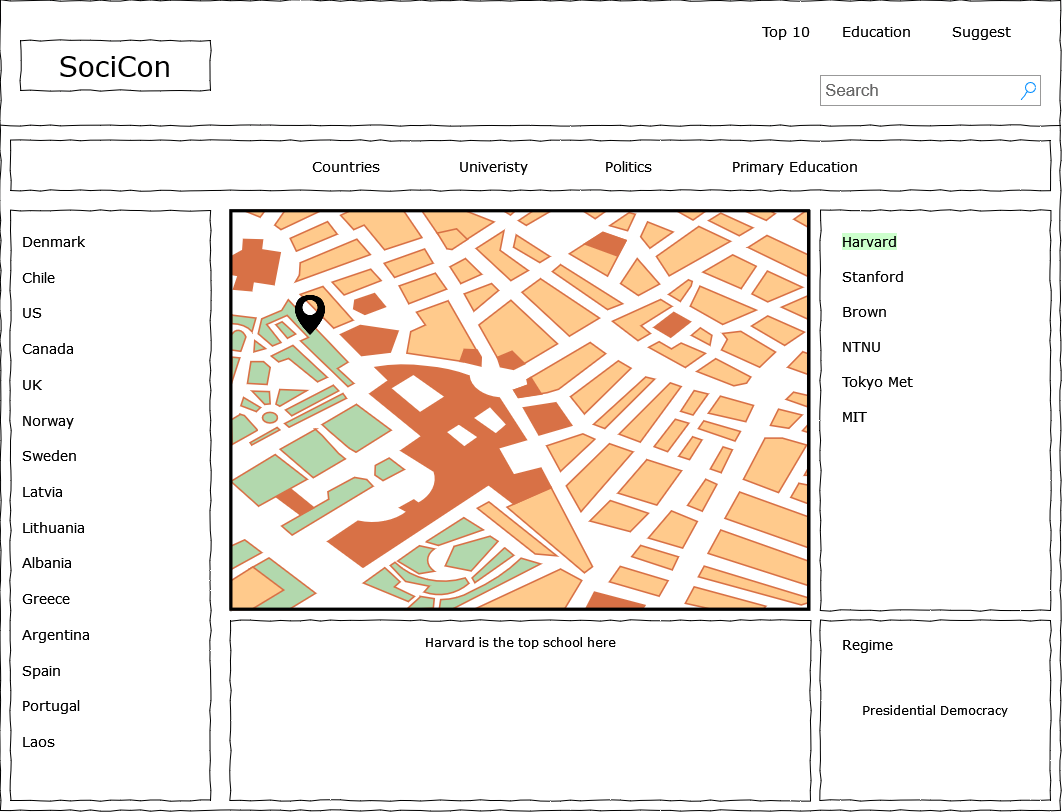
\includegraphics[width=\textwidth]{images/milepael1/forsideBigdata.png}
\end{figure}
